% \begin{tcolorbox}[title=TODO]
% Developed architecture / system design / implementation: 1/3
% \begin{itemize}
% \item start with a theoretical approach
% \item describe the developed system/algorithm/method from a high-level point of view
% \item go ahead in presenting your developments in more detail
% \end{itemize}
% \end{tcolorbox}
\section{Image Size}
\label{sec:image-size}
Reducing the image size of an operating system is crucial for updating IoT devices
with low bandwidth, regardless of which update methodology is used.
In environments where network connectivity is limited or expensive,
smaller image sizes result in faster and more efficient updates.

We need to create a minimal operating system image that is significantly smaller
than Microsoft's recommended \textit{Ubuntu 22.04}, while still being able to run the
\textit{Azure IoT Edge} runtime and the required software. This image must also
feature the efficient update mechanism of \textit{reUpNix}.

However, \textit{Azure Iot Edge} is not officially supported on \textit{NixOS}
by Microsoft and there is no \textit{Nix} package available. Therefore, we need
to create a \textit{Nix} package for \textit{Azure IoT Edge} and all of its
dependencies from the publicly available source code. This is a crucial step, since
without a working \textit{Azure IoT Edge} runtime, we cannot draw any meaningful
conclusions for updating \ac{IIoT} devices using \textit{Azure IoT}.

To create the \textit{Nix} packages, we need to understand the dependencies of
\textit{Azure IoT Edge} and how to package them. As we can see in figure
\ref{fig:dependency-tree}, \textit{Azure IoT Edge} runtime has a tree of dependencies,
many of which are common to \textit{Linux} systems, which means that we can
utilize the over 80,000 already existing \textit{Nix} packages to meet
those dependencies.
\clearpage

\begin{figure}[H]
    \centering
    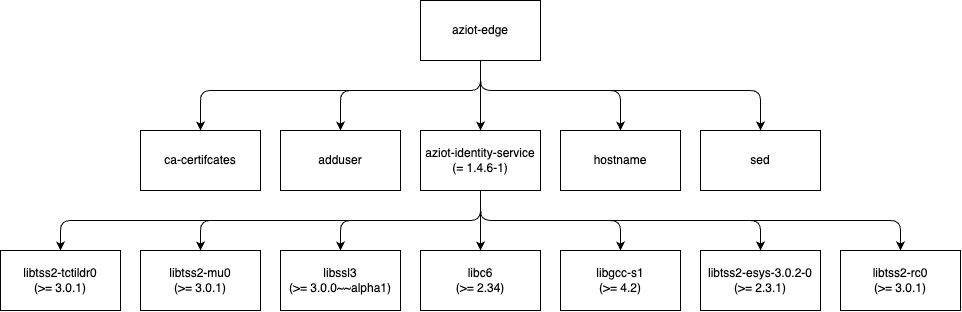
\includegraphics[width=\textwidth]{fig/dependecy-tree.drawio.png}
    \caption{Azure IoT Edge Dependency Tree}
    \label{fig:dependency-tree}
\end{figure}


Once we have created a minimal operating system image using \textit{reUpNix}, we
need to measure the size of the image. Then repeat the measurements for
\textit{Ubuntu 22.04}, \textit{Yocto Kirkstone} and \textit{NixOS}, such that
we are able to compare the operating systems and draw a conclusion.

\subsection{Hypothesis}
Since \textit{reUpNix} has already shown to be able to reduce the size of the
operating system image \cite{gollenstede:23:lctes}, we hypothesize that the
image size of \textit{reUpNix} including the \textit{Azure IoT Edge} runtime
will also be significantly smaller than the image size of \textit{NixOS},
\textit{Ubuntu 22.04}, and \textit{Yocto Kirkstone}.


\section{Update size}
\label{sec:update-size}
When updating the operating system with an A/B partition schema, the entire
image needs to be downloaded and written to a secondary partition. In this
\ac{OTA} scenario the size of the operating system image is critical, as we have
already discussed in chapter \ref{sec:image-size}.
However, if we adapt a different methodology than an A/B partition schema
for updating the operating system, we can potentially reduce the update size
drastically.

We want to establish if using \textit{reUpNix}'s differential updates as the
update mechanism for an \ac{IIoT} device with \textit{Azure IoT Edge}
will result in a smaller update size in comparison to using an A/B partition schema with
\textit{Ubuntu 22.04} and \textit{Yocto Kirkstone}. To do so, we need to create
an update for a \textit{reUpNix} system, in which we upgrade the majority
of software packages installed, so that it is comparable to a distribution upgrade
of \textit{Ubuntu 22.04} and \textit{Yocto Kirkstone}.

Importantly, the created updates, regardless for which \ac{OS}, must all be
able to be installed using the \textit{Azure IoT Update Service} and respective
\textit{Azure IoT Update Agent}. Since the \textit{Azure IoT Update Agent} is
not officially supported on \textit{NixOS}, we need to create a \textit{Nix} package
for the \textit{Azure IoT Update Agent} and all of its dependencies.

\subsection{Hypothesis}

Since \textit{reUpNix} uses a differential approach to updating the operating
system and therefore only transmits the changes between the old and the new
version, we hypothesize that the update size of \textit{reUpNix} will be
significantly smaller than the update size of \textit{Ubuntu 22.04} and
\textit{Yocto Kirkstone}. It was already shown that the update size of
\textit{reUpNix} is significantly smaller than the update size of \textit{NixOS}
\cite{gollenstede:23:lctes}, so we expect this to be also true for a variant
of \textit{reUpNix} including the \textit{Azure IoT Edge} runtime.

\section{Time To Recover}
Customers of certain industries require high availability and reliability for
their \ac{IIoT} devices and applications. These availability requirements
are commonly legally and formally negotiated in an \ac{SLA} between
the customer and a service provider \cite{msdoc-slas}. An important consideration
for service providers to achieve high availability is the boot time of the
\ac{OS}. However, for this experiment the time to recover is considered,
instead of the actual boot time of the \ac{OS}. For this experiment, we define the
time to recover as the time until Azure IoT Edge runtime is operable again after
an unexpected reboot.

We argue that the time until operability is more relevant for service providers
when defining \ac{SLO}, since the boot process contains several steps that are
outside of the scope of the \ac{OS}, for example, hardware, BIOS/UEFI or the boot
loader \cite{almesberg}.

% \subsection{Setup}
For this experiment, we will restart the system by sending a \textit{reboot} system
call to the kernel with the \code{reboot} command line tool \cite{man-reboot}.
In order to execute the command, a \ac{SSH} connection to the target machine
needs to be established.

\clearpage

\begin{figure}[H]
    \centering
    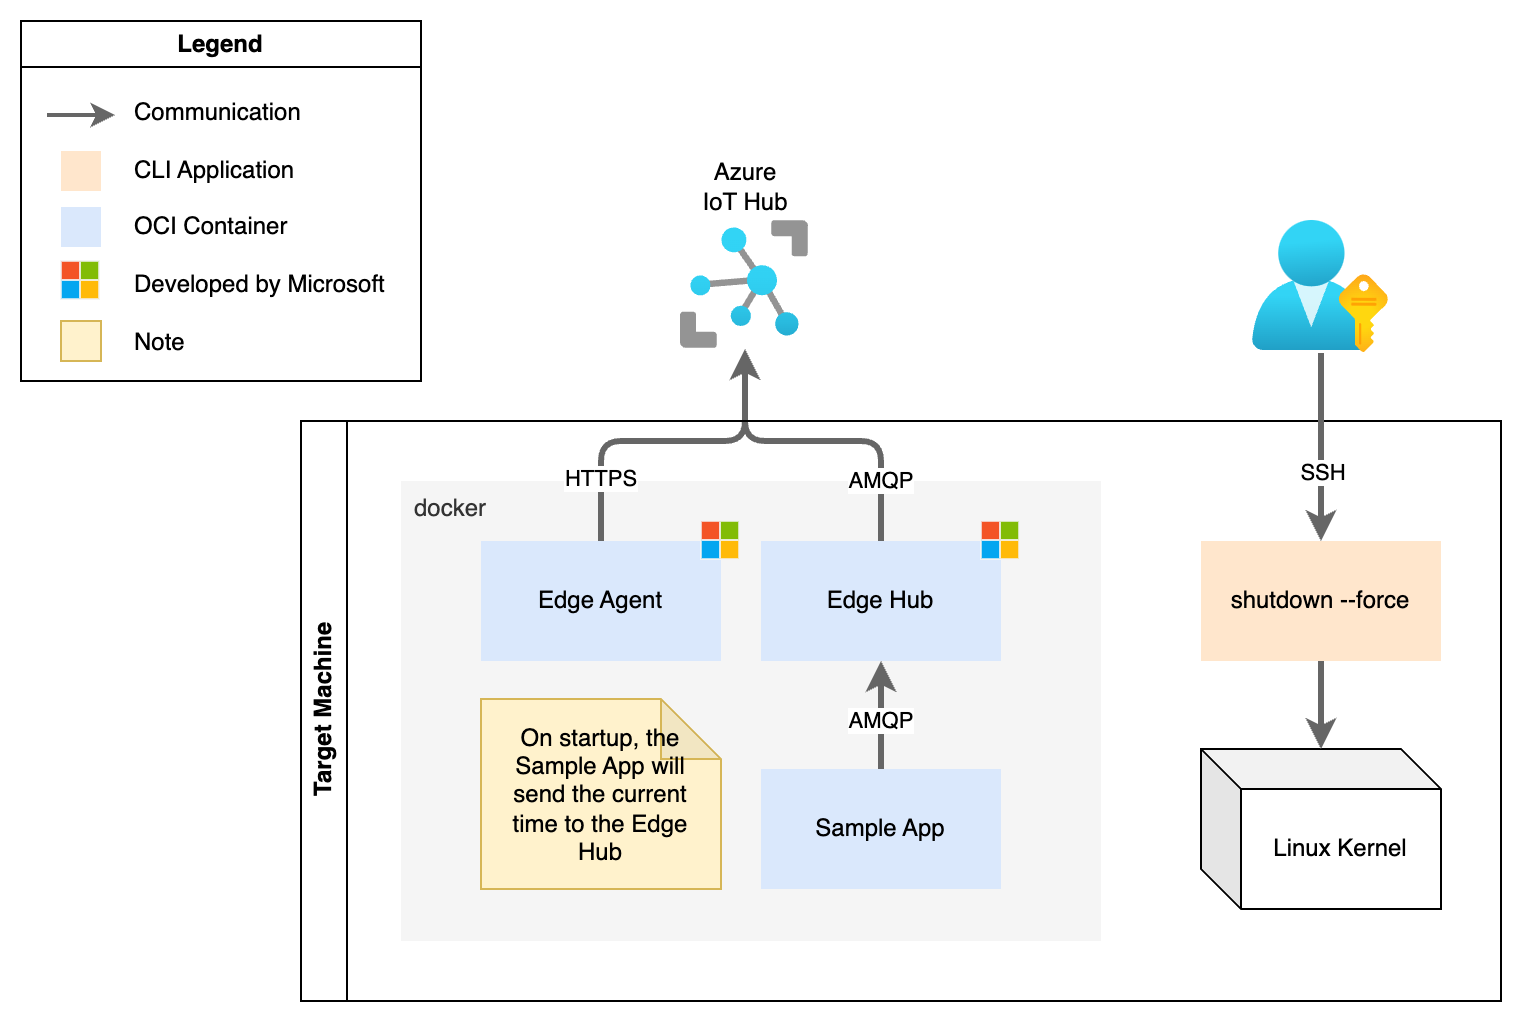
\includegraphics[width=0.75\textwidth]{fig/reboot-setup.drawio.png}
    \caption{Time To Recover Experiment Overview}
\end{figure}

\noindent
Just before the system is rebooted, the current time will be printed.
After the \ac{OS} rebooted and the Azure IoT Edge runtime has started, a
sample app will send the current time to the Azure IoT Hub via the Azure IoT Edge
Hub, where it can be retrieved. The full shell command can be seen in listing
\ref{lst:reboot-command}.
\\

\begin{lstlisting}[
    caption=Shell Commands For Time To Recover Experiment,
    label=lst:reboot-command]
date +%s \
&& reboot
\end{lstlisting}

\noindent
When comparing the first timestamp ($t_0$) from the shell command output with the second
timestamp ($t_1$) from the \textit{Azure IoT Hub}, the time to recover can be calculated
as the delta between those two timestamps:

\begin{equation}
    T := |t_1 - t_0|
\end{equation}
However, since rebooting the \ac{OS} is a process with many variances, the experiment
must be repeated multiple times. If we repeat the experiment $n$ times, where
$T_i$ represents the result of the $i$-th repetition, we can calculate
a mean value for $T$ as:

\begin{equation}
    \mu := \frac{\sum_{i=1}^{n}T_i}{n}
\end{equation}

\noindent
And the standard deviation for $T$ as:

\begin{equation}
   \sigma := \sqrt{\frac{\sum_{i=1}^{n}((T_i - \mu)^2}{n}}
\end{equation}

\noindent
Finally, the standard error for $T$ as:

\begin{equation}
    s := \frac{\sigma}{\sqrt{n}}
\end{equation}

\noindent
This experiment must be repeated until the standard error is low enough
to have a confident mean value for each \ac{OS}.

\subsection{Hypothesis}
Our hypothesis is that the time to recover will be very similar for all
\ac{OS}s. Since they all run \textit{Linux}, the Azure IoT Edge runtime and
a similar set of software, such as \textit{systemd} and \ac{SSH}. However, due
to the reduced size of \textit{reUpNix}, we may see a slight advantage in the
time to recover, since the \ac{OS} has to load less data from the disk. Further,
\textit{reUpNix} has a minified kernel and a reduced set of kernel modules.

\section{Container Updates}
\label{sec:container-updates}
When using Azure IoT Edge, \ac{IIoT} applications are deployed as containers because
they change more frequent than the entire \ac{OS}. When a module is updated
with a new deployment manifest, Azure IoT Edge retrieves any new container
images that are not present on the device. It uses a \ac{UDS} to communicate
with the container runtime, to pull the image. The same can be manually achieved
with the \code{docker pull} command, when using Docker as the container runtime.

In an \ac{IIoT} scenario, where network connectivity is limited or expensive,
we want to avoid pulling entire container images when only a few files have
changed. Since the \textit{Nix store} has a pretty efficient mechanism for
deduplicating files, we want to investigate if we can use \textit{reUpNix}'s
update mechanism to update containers in a more efficient way.

Our proposed approach is to pull and unpack the container images during the built
process of the \ac{OS}, letting \textit{Docker} populate the \textit{/var/lib/docker}
directory inside a build-sandbox with the container image layers and meta data.
Then storing the result in the \textit{Nix store} and including the
\textit{Nix store} object in to the system configuration. On boot, the
\textit{/var/lib/docker} directory is then mounted from the \textit{Nix store}
with an overlay, so that the container runtime can access the container images.

We need to verify by comparing the \textit{reUpNix} update size to the size of the container layers,
which are updated by a docker pull, that this approach reduces the data transmitted.

\subsection{Hypothesis}
Our hypothesis is that updating containers with \textit{reUpNix}'s differential
update mechanism will be more efficient than updating them with Azure IoT Edge or
the \code{docker pull} command. This is due to the fact that, if the uppermost
layer of a container image only contains minimal changes (e.g. only a few
changed files), the differential update will only transmit the changed files in
that layer instead of the entire layer.
